
\chapter{Numerical Validation}
\label{chp:NumMethodComp}

\section{Measuring Convergence and Conservation}
The assessment of the accuracy of the numerical methods will be assessed in this chapter by investigating their convergence and conservation properties. To do this will require some measure of the distance between numerical solutions and the analytic solution to determine the convergence of the method, while for conservation some measure of the total of quantity in our numerical solution is needed. We introduce our notation for these measures and describe their calculation here.

\subsection{Measures of Convergence}
By measuring the relative difference between our numerical solutions and the analytic solution we can observe the convergence of all numerical methods as $\Delta x$ varies. To do this we use the $L_1$ vector norm, considering the analytic solutions only at the grid points. For a quantity $q$ the vectors of its values $\vecn{q}$ at the grid locations $x_j$ and the corresponding numerical solution at those locations $\vecn{q^*}$ the $L_1$ norm is
\begin{equation}
L_1(q) =  \left\lbrace \begin{array}{c r} 
\dfrac{||\vecn{q^*} - \vecn{q}||_{1}}{||\vecn{q}||_{1}} & ||\vecn{q}||_{1} > 0 \\ \\
{||\vecn{q^*}||_{1}} & ||\vecn{q}||_{1} = 0  \end{array}\right. . 
\label{eqn:L1qdef} 
\end{equation}

When no analytic solution is present, we can compare the distance between two numerical solutions to gain some insight into how the sequence of numerical solutions is behaving. We do this in a similar way as \eqref{eqn:L1qdef} and compare the $L_1$ norm of the two numerical solutions vectors $\vecn{q^*}$ and $\vecn{q'}$. We have constructed our grids to accommodate this, and as such we vary $\Delta x$ by dividing by powers of $2$ this ensures that grid locations generated by the larger $\Delta x$ values are also present in the grid generated by the smaller $\Delta x$ value, and so we can just compare $\vecn{q^*}$ and $\vecn{q'}$ on the common grid points generated by the larger $\Delta x$. When we do this we denote it as $L^*_1$.


\subsection{Measures of Conservation}
The conservation properties of the methods as $\Delta x$ varies can be observed by calculating the total of the quantity in the numerical solution $\mathcal{C}^*\left({\vecn{q^*}}\right)$ and comparing it to the total of the quantity $\mathcal{C}\left({q(x,0)} \right)$ analytically. We do this again using a relative measure $C_1$ 
\begin{equation}
C_1(q) =  \left\lbrace \begin{array}{c r} 
\dfrac{|\mathcal{C}^*\left({\vecn{q^*}}\right) - \mathcal{C}\left({q(x,0)} \right)| }{|\mathcal{C}\left({q(x,0)} \right)|} & |\mathcal{C}\left({q(x,0)} \right)| > 0 \\ \\
|\mathcal{C}^*\left({\vecn{q^*}}\right)| & |\mathcal{C}\left({q(x,0)} \right)| = 0  \end{array}\right. . 
\label{eqn:C1qdef} 
\end{equation}
$\mathcal{C}^*\left({\vecn{q^*}}\right)$ was calculated by 3 point Gaussian quadrature over the $j^{th}$ cell and summing these integral for all cells. The three points needed to perform the Gauss quadrature were calculated by interpolating the $j^{th}$ cell using a quartic that fits the nodal values $q_{j-2}$,$q_{j-1}$,$q_{j}$,$q_{j+1}$ and $q_{j+2}$. The Guassian quadrature using three points is $5^{th}$ order accurate and the interpolation by quartics will be $5^{th}$ order accurate for the quantity $q$ and $4^{th}$ order accurate for $\partial q \partial x$. Therefore, the error introduced by the calculation of $\mathcal{C}^*\left({\vecn{q^*}}\right)$ for the mass, momentum, $G$ and $\mathcal{H}$ will be much smaller than the error introduced by the numerical solvers.

In some cases $\mathcal{C}\left({q(x,0)} \right)$ may be difficult to derive and instead we compare $\mathcal{C}^*\left({\vecn{q^*}}\right)$ and the total quantity $q$ at $t=0$ $\mathcal{C}^*\left({\vecn{q}^0}\right)$. Comparing these we get 
\begin{equation}
C^*_1(q) =  \left\lbrace \begin{array}{c r} 
\dfrac{|\mathcal{C}^*\left({\vecn{q^*}}\right) - \mathcal{C}^*\left({\vecn{q}^0}\right)| }{|\mathcal{C}^*\left({\vecn{q}^0}\right)|} & |\mathcal{C}^*\left({\vecn{q}^0}\right)| > 0 \\ \\
|\mathcal{C}^*\left({\vecn{q^*}}\right)| & |\mathcal{C}^*\left({\vecn{q}^0}\right)| = 0  \end{array}\right. . 
\label{eqn:C*1qdef} 
\end{equation}


\section{Analytic Solutions}

\subsection{Soliton}
%C1, H1 and L1
The soliton is an analytic solution of the Serre equations, it is a travelling wave solution and occurs in the limit [] for the cnoidal wave family of solutions. The soliton travels without deformation due to a balance between the nonlinear effects that causes deeper water to travel faster and the dispersive effects that causes longer waves to travel faster. []

We numerically solved the Serre equations using \eqref{eqn:Solitondefhub} and \eqref{eqn:SolitondefG} with $a_0 = 1m$ , $a_0 = 0.7m$ and $g= 9.81m/s^2$ at $t=0s$ as initial conditions. The spatial domain was $[-250m,250m]$ and the problem was solved until $t= 50s$. This was done for all numerical methods across a range of $\Delta x$ values that had the following form $\Delta x = 100 / 2^k m$ with $k \in  \left[6,7, \dots,19\right]$ and we chose $\Delta t = Cr / \sqrt{g\left(a_0 + a_1\right)}$ to satisfy the CFL condition with CFL number $Cr = 0.5$. For $\text{FDVM}_2$ and $\text{FEVM}_2$ we used $\theta  = 1.2$ as the limiting parameter in the generalised minmod limiter. 

The particular soliton problem was chosen as the non-linearity parameter $\epsilon = a_1 / a_0 = 0.7$ is beneath the breaking threshold. The spatial domain was chosen so that there were no effects from the boundary throughout the numerical solution and the final time allowed for many time-steps to be performed. 

\subsubsection{Results}
%mention FEVM first?
An example numerical solution with $\Delta x = {100} / {2^{11}}m$ from all methods was plotted in Figure \ref{fig:SolitonExAll} against the analytic solution at $t= 50s$. We have only plotted an illustrative amount of the points in the numerical solution. From these plots it is clear that $\text{FDVM}_1$ performs significantly worse than the other methods of accurately reproducing the numerical solution, even for relatively fine grids where the wave is captured by more than $200$ cells. This is primarily due to the numerical diffusion introduced by the method, which has caused the soliton to decrease in amplitude and widen significantly. The higher-order numerical methods all accurately replicate the analytic solution, with insignificant differences in these plots.

\begin{figure}
	\centering
	\begin{subfigure}{0.5\textwidth}
		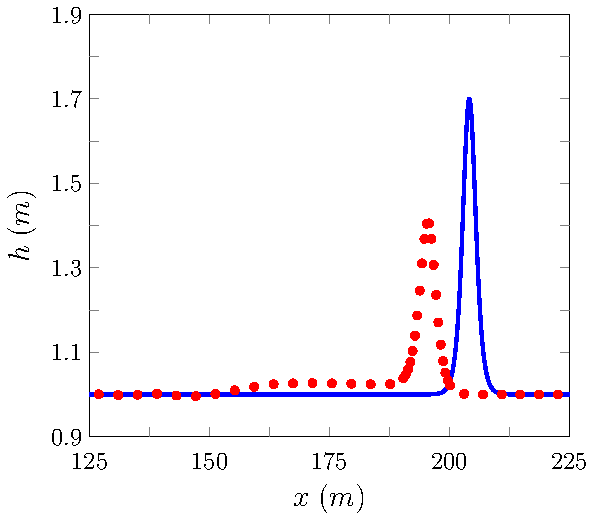
\includegraphics[width=\textwidth]{./chp5/figures/Analytic/Soliton/Example/FDVM1.pdf}
		\subcaption{$\text{FDVM}_1$}
		\vspace{0.5cm}
	\end{subfigure}%
	\begin{subfigure}{0.5\textwidth}
		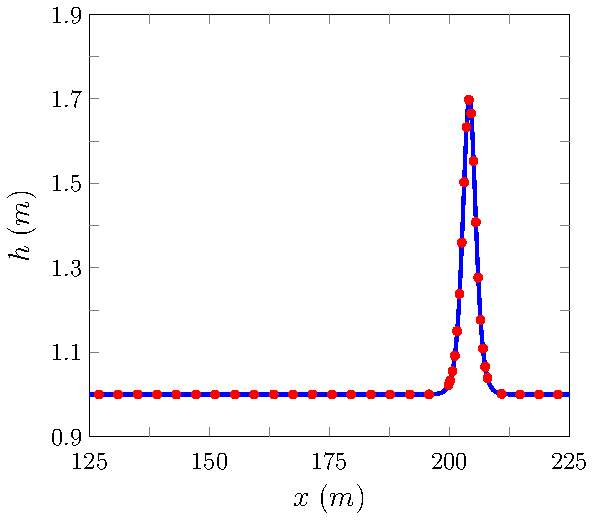
\includegraphics[width=\textwidth]{./chp5/figures/Analytic/Soliton/Example/FDVM2.pdf}
		\subcaption{$\text{FDVM}_2$}
		\vspace{0.5cm}
	\end{subfigure}
	\begin{subfigure}{0.5\textwidth}
		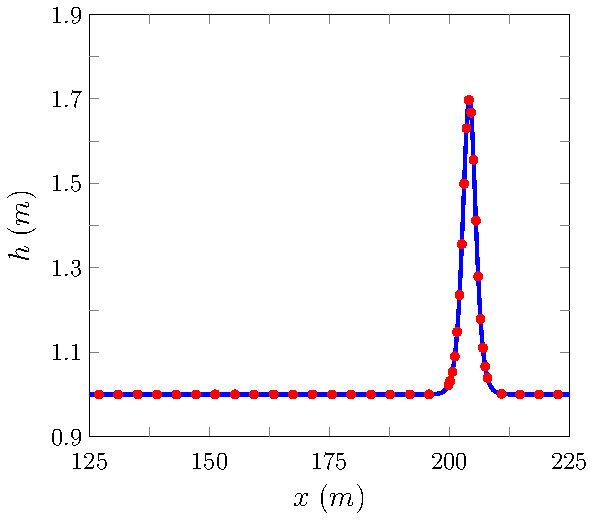
\includegraphics[width=\textwidth]{./chp5/figures/Analytic/Soliton/Example/FEVM2.pdf}
		\subcaption{$\text{FEVM}_2$}
		\vspace{0.5cm}
	\end{subfigure}%
	\begin{subfigure}{0.5\textwidth}
		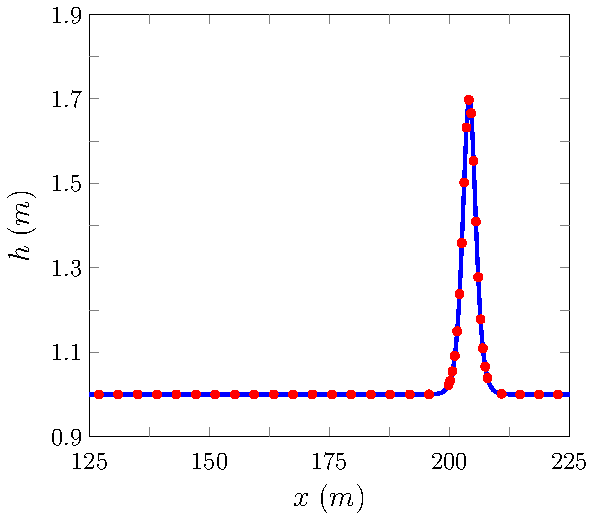
\includegraphics[width=\textwidth]{./chp5/figures/Analytic/Soliton/Example/FDVM3.pdf}
		\subcaption{$\text{FDVM}_3$}
		\vspace{0.5cm}
	\end{subfigure}
	\begin{subfigure}{0.5\textwidth}
		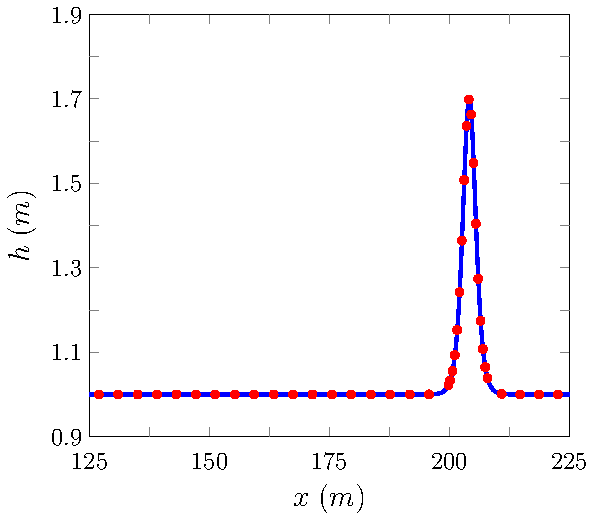
\includegraphics[width=\textwidth]{./chp5/figures/Analytic/Soliton/Example/D.pdf}
		\subcaption{$\mathcal{D}$}
		\vspace{0.5cm}
	\end{subfigure}%
	\begin{subfigure}{0.5\textwidth}
		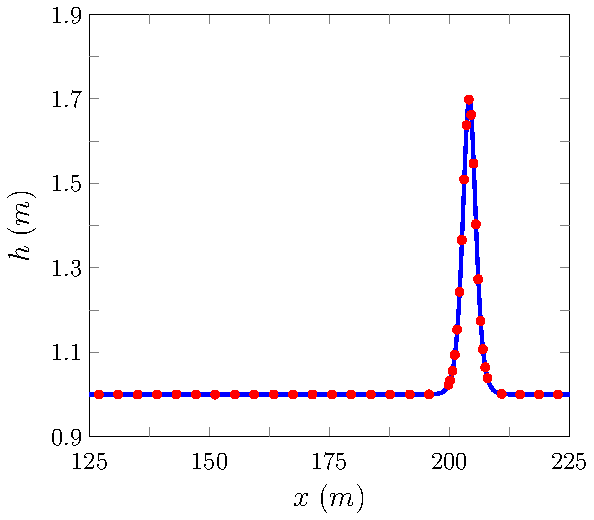
\includegraphics[width=\textwidth]{./chp5/figures/Analytic/Soliton/Example/W.pdf}
		\subcaption{$\mathcal{W}$}
		\vspace{0.5cm}
	\end{subfigure}
	\caption{Comparison of the analytic solution ({\color{blue} \solidrule}) and numerical solution with $\Delta x = {100} / {2^{11}}m$ ({\color{red} $\bullet$}) for the soliton problem at $t=50s$ for all methods.}
	\label{fig:SolitonExAll}
\end{figure}


The $L_1$ norm was measured for $h$, $u$ and $G$ for all numerical solutions and was plotted against $\Delta x$ for all numerical methods in Figure \ref{fig:SolitonL1All}. All numerical methods demonstrate convergence for all quantities. We also see that all numerical methods demonstrate the appropriate order of accuracy in the convergence. This agrees with our analysis of these methods applied to the linearised Serre equations in Chapter []. 
%Compare the L_1 norms for the second order methods, the round off error
\begin{figure}
	\centering
	\begin{subfigure}{0.5\textwidth}
		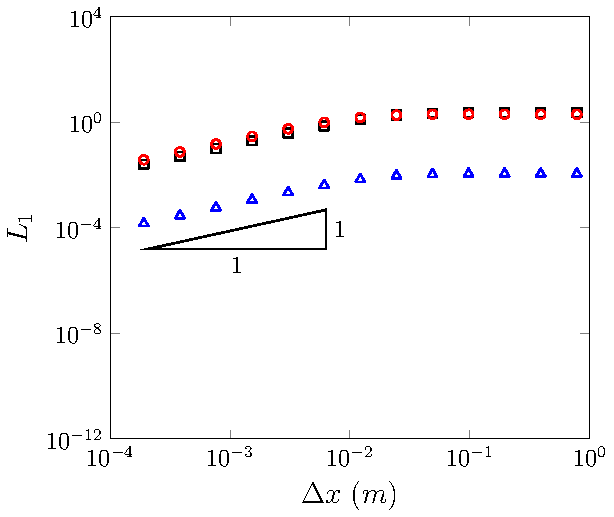
\includegraphics[width=\textwidth]{./chp5/figures/Analytic/Soliton/L1/FDVM1.pdf}
		\subcaption{$\text{FDVM}_1$}
		\vspace{0.5cm}
	\end{subfigure}%
	\begin{subfigure}{0.5\textwidth}
		\includegraphics[width=\textwidth]{./chp5/figures/Analytic/Soliton/L1/FDVM2.pdf}
		\subcaption{$\text{FDVM}_2$}
		\vspace{0.5cm}
	\end{subfigure}
	\begin{subfigure}{0.5\textwidth}
		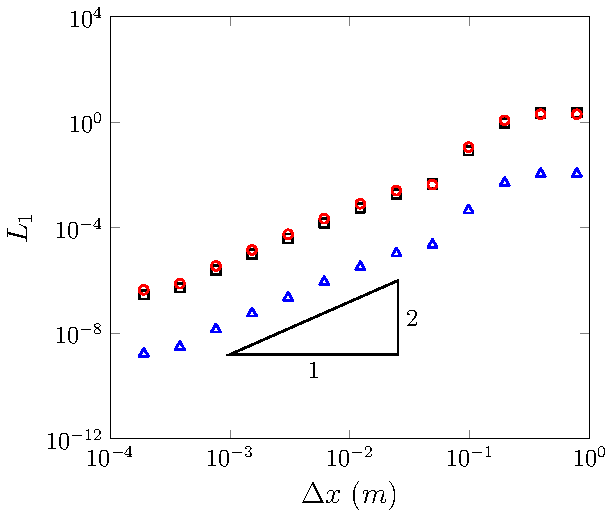
\includegraphics[width=\textwidth]{./chp5/figures/Analytic/Soliton/L1/FEVM2.pdf}
		\subcaption{$\text{FEVM}_2$}
		\vspace{0.5cm}
	\end{subfigure}%
	\begin{subfigure}{0.5\textwidth}
		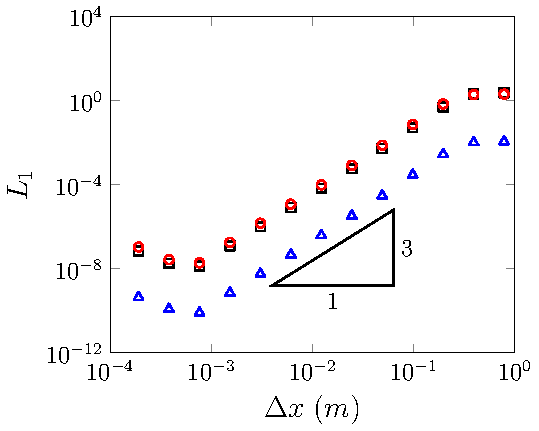
\includegraphics[width=\textwidth]{./chp5/figures/Analytic/Soliton/L1/FDVM3.pdf}
		\subcaption{$\text{FDVM}_3$}
		\vspace{0.5cm}
	\end{subfigure}
	\begin{subfigure}{0.5\textwidth}
		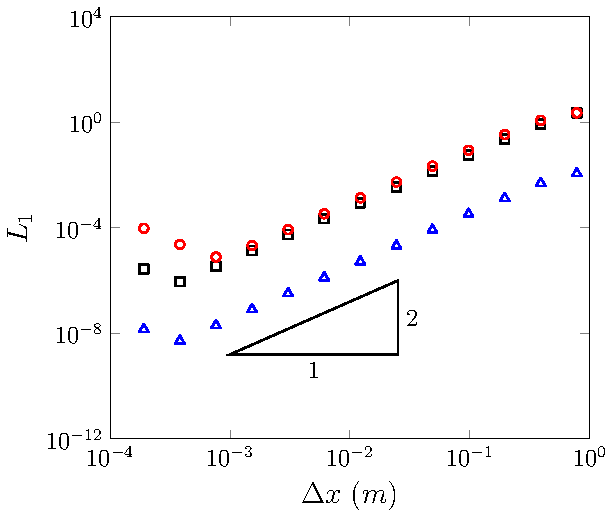
\includegraphics[width=\textwidth]{./chp5/figures/Analytic/Soliton/L1/D.pdf}
		\subcaption{$\mathcal{D}$}
		\vspace{0.5cm}
	\end{subfigure}%
	\begin{subfigure}{0.5\textwidth}
		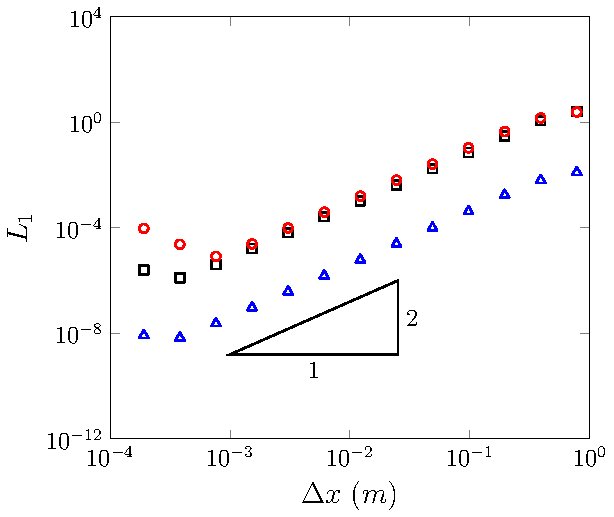
\includegraphics[width=\textwidth]{./chp5/figures/Analytic/Soliton/L1/W.pdf}
		\subcaption{$\mathcal{W}$}
		\vspace{0.5cm}
	\end{subfigure}
	\caption{Convergence plots as measured by the $L_1$ norm for $h$ (\trianglet{blue}), $u$ (\squaret{black}) and $G$ (\diamondt{red}) for the soliton problem for all methods.}
	\label{fig:SolitonL1All}
\end{figure}
%
The $C_1$ norm was measured for mass ($h$), momentum ($uh$), $G$ and $\mathcal{H}$ and plotted in Figure \ref{fig:SolitonC1All}. From these plots we can see that all methods conserve mass at round-off error as long as $\Delta x$ isn't too large, in this case requiring $\Delta x < 0.5m$. Since the FD methods perform just as well at conserving mass as the FDVM and FEVM, this suggests that a finite volume method for the conservation law is not necessary to conserve mass for the soliton problem.

The conservation of momentum is significantly above round-off error, and for all numerical methods decreases at the rate determined by the order of accuracy or better. For the FDVM and the FEVM this is not surprising as $u$ is calculated from the elliptic equation, which is not strictly conservative for the momentum. While for the FD methods which solve the momentum equation directly do not conserve momentum as their are finite difference methods and so are not necessarily conservative. Given the results for the $L_1$ norm, one might expect that the $C_1$ norm would have the same rate of decrease. However, given that the a quantity can be conserved with a large $L_1$ norm, for instance if translations of the solution we should only expect that the rate of decrease in $C_1$ is the same or larger than in $L_1$. 

For the conservation of $G$ we see that the case is very similar to the momentum, except for the FEVM which conserves $G$ at round-off error as long as $\Delta x$ isn't large. This implies that the FD used to solve the elliptic equation while resulting in smaller errors of $u$ breaks the conservation of $G$ implied by the conservation equations []. Therefore, we require a FEM to solve the elliptic equation so that our scheme conserves the conservative quantities $h$ and $G$.

The conservation of the Hamiltonian also decreases at the rate given by the order of accuracy of the method or better.
%comment on individual features of the conservation plots  
%
\begin{figure}
	\centering
	\begin{subfigure}{0.5\textwidth}
		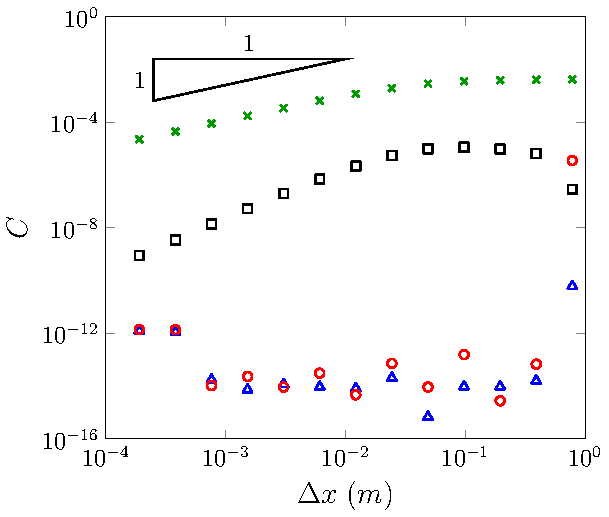
\includegraphics[width=\textwidth]{./chp5/figures/Analytic/Soliton/C1/FDVM1.pdf}
		\subcaption{$\text{FDVM}_1$}
		\vspace{0.5cm}
	\end{subfigure}%
	\begin{subfigure}{0.5\textwidth}
		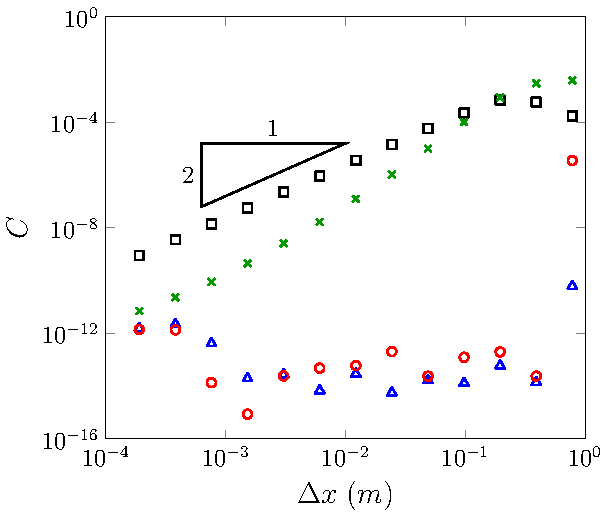
\includegraphics[width=\textwidth]{./chp5/figures/Analytic/Soliton/C1/FDVM2.pdf}
		\subcaption{$\text{FDVM}_2$}
		\vspace{0.5cm}
	\end{subfigure}
	\begin{subfigure}{0.5\textwidth}
		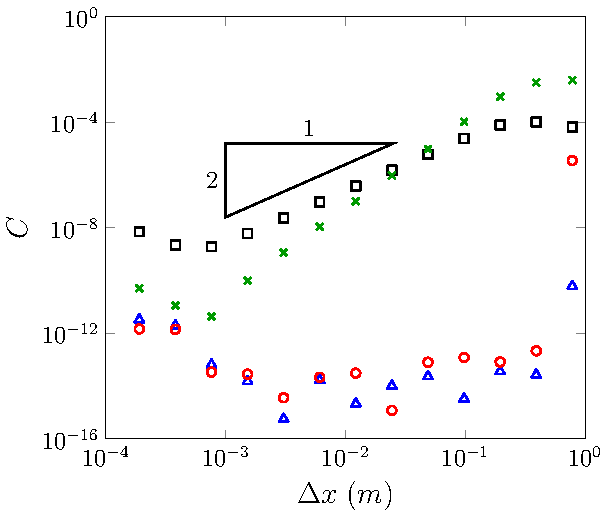
\includegraphics[width=\textwidth]{./chp5/figures/Analytic/Soliton/C1/FEVM2.pdf}
		\subcaption{$\text{FEVM}_2$}
		\vspace{0.5cm}
	\end{subfigure}%
	\begin{subfigure}{0.5\textwidth}
		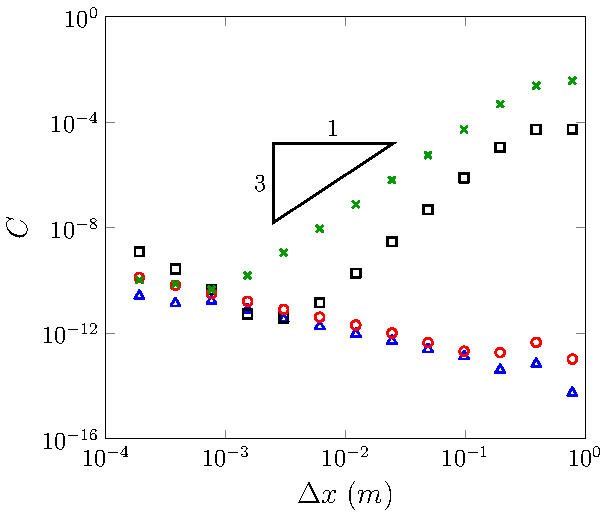
\includegraphics[width=\textwidth]{./chp5/figures/Analytic/Soliton/C1/FDVM3.pdf}
		\subcaption{$\text{FDVM}_3$}
		\vspace{0.5cm}
	\end{subfigure}
	\begin{subfigure}{0.5\textwidth}
		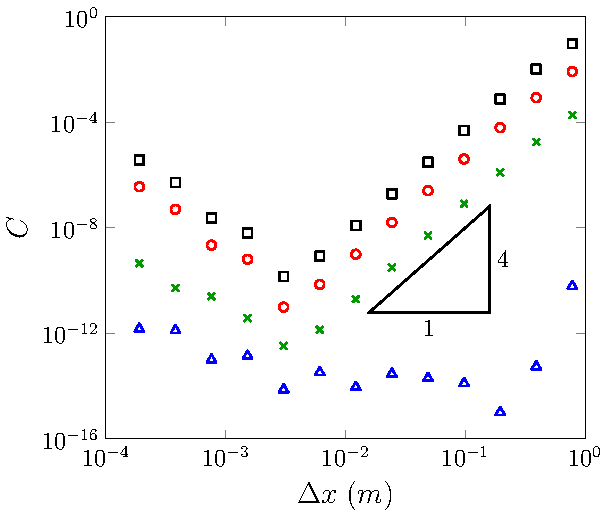
\includegraphics[width=\textwidth]{./chp5/figures/Analytic/Soliton/C1/D.pdf}
		\subcaption{$\mathcal{D}$}
		\vspace{0.5cm}
	\end{subfigure}%
	\begin{subfigure}{0.5\textwidth}
		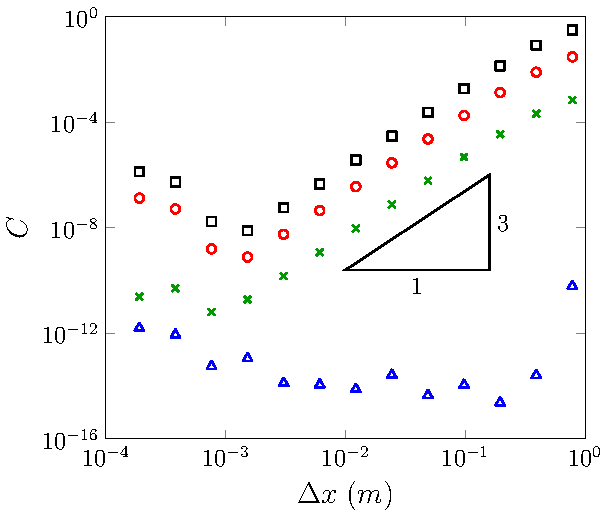
\includegraphics[width=\textwidth]{./chp5/figures/Analytic/Soliton/C1/W.pdf}
		\subcaption{$\mathcal{W}$}
		\vspace{0.5cm}
	\end{subfigure}
	\caption{Conservation plots as measured by $C_1$ for $h$ (\trianglet{blue}), $uh$ (\squaret{black}), $G$ (\diamondt{red}) and $\mathcal{H}$ (\circlet{green!80!black}) for the soliton problem for all methods.}
	\label{fig:SolitonC1All}
\end{figure}

\subsection{Lake at Rest}
%C1, H1 and L1

\begin{subequations}
	\begin{align}
	&h(x,t) =  \max\left(a_0 - b(x),0\right)\\
	&u(x,t) = 0 \\
	&b(x) = a_1 \sin\left(a_2 x\right) \\
	\end{align}
\end{subequations}

\begin{equation}
G(x,t) =0 
\end{equation}

Conservation
\begin{align}
&\int h(x,0) \; dx = \left\lbrace  \begin{array}{c c}
a_0 x + \dfrac{a_1 \cos\left(a_2 x\right)}{a2} & a_0 > a_1 \sin\left(a_2 x\right)
\\ 0 & \text{otherwise}
\end{array}\right. \\
&\int u(x,0)h(x,0) \; dx =0
\end{align}

\begin{multline}
\int G(x,0) \; dx = 0
\end{multline}

\begin{multline}
\int \mathcal{H}(x,0) \; dx =  \\\frac{1}{2} \left(g\int\left[h(x,0)\right]^2  + 2g\int h(x,0)b(x) \right)
\end{multline}


\begin{align}
&\int \left[h(x,0)\right]^2 \; dx = \left\lbrace  \begin{array}{c c}
\dfrac{1}{4a_2} \left(2a_2 x\left(2a_0^2 + a_1^2\right) + 8 a_0 a_1 \cos\left(c_2 x\right)- a_1^2\sin\left(2a_2 x\right)\right) & a_0 > a_1 \sin\left(a_2 x\right)
\\ 0 & \text{otherwise}
\end{array}\right. 
\end{align}

\begin{align}
&\int h(x,0)b(x)\; dx = \left\lbrace  \begin{array}{c c}
\dfrac{a_1}{4a_2}\left(a_1\left(\sin\left(2a_2x\right) - 2 a_2 x\right) - 4 a_0 \cos\left(a_2 x\right)\right)  & a_0 > a_1 \sin\left(a_2 x\right)
\\ 0 & \text{otherwise}
\end{array}\right. 
\end{align}

\begin{figure}
	\centering
	\begin{subfigure}{0.5\textwidth}
		\includegraphics[width=\textwidth]{./chp5/figures/Analytic/LakeAtRest/Example/FDVM2.pdf}
		\subcaption{$\text{FDVM}_2$}
	\end{subfigure}%
	\begin{subfigure}{0.5\textwidth}
		\includegraphics[width=\textwidth]{./chp5/figures/Analytic/LakeAtRest/Example/FEVM2.pdf}
		\subcaption{$\text{FEVM}_2$}
	\end{subfigure}
	\caption{ Plot of the water surface ({\color{blue} \solidrule}) laying on the bed profile ({\color{green!60!black} \solidrule}) from the numerical solutions with $\Delta x = {\text{width}} / {2^{12}}m$ at $t = 10s$.}
	\label{fig:LakeAtRestExAll}
\end{figure}

\begin{figure}
	\centering
	\begin{subfigure}{0.5\textwidth}
		\includegraphics[width=\textwidth]{./chp5/figures/Analytic/LakeAtRest/L1/FDVM2.pdf}
		\subcaption{$\text{FDVM}_2$}
	\end{subfigure}%
	\begin{subfigure}{0.5\textwidth}
		\includegraphics[width=\textwidth]{./chp5/figures/Analytic/LakeAtRest/L1/FEVM2.pdf}
		\subcaption{$\text{FEVM}_2$}
	\end{subfigure}
	\caption{Convergence plots as measured by the $L_1$ norm for $h$ (\trianglet{blue}), $u$ (\squaret{black}) and $G$ (\diamondt{red}) for the lake at rest problem for all methods.}
	\label{fig:LakeAtRestL1All}
\end{figure}

\begin{figure}
	\centering
	\begin{subfigure}{0.5\textwidth}
		\includegraphics[width=\textwidth]{./chp5/figures/Analytic/LakeAtRest/C1/FDVM2.pdf}
		\subcaption{$\text{FDVM}_2$}
	\end{subfigure}%
	\begin{subfigure}{0.5\textwidth}
		\includegraphics[width=\textwidth]{./chp5/figures/Analytic/LakeAtRest/C1/FEVM2.pdf}
		\subcaption{$\text{FEVM}_2$}
	\end{subfigure}
	\caption{Conservation plots as measured by $C_1$ for $h$ (\trianglet{blue}), $uh$ (\squaret{black}), $G$ (\diamondt{red}) and $\mathcal{H}$ (\circlet{green!80!black}) for the lake at rest problem for all methods.}
	\label{fig:LakeAtRestC1All}
\end{figure}

\section{Forced Solutions}
%only L1

\subsection{Travelling Gaussian}
\begin{equation}
h(x,t) = a_0 + a_1\exp\left(-\dfrac{ \left(\left(x - a_2t\right) - a_3 \right)^2}{2a_4}\right)
\end{equation}
\begin{equation}
u(x,t) = a_5\exp\left(-\dfrac{ \left(\left(x - a_2t\right) - a_3 \right)^2}{2a_4}\right)
\end{equation}
\begin{equation}
b(x) = a_6\sin\left(a_7 x\right)
\end{equation}

%With $a_0 = 1$ or $a_0 = 0$.
%$a_1 = 0.5$
%$a_2 = 1$
%$a3 = -20$
%$a4 = 1$
%$a5 = a1$
%$a6 = 1$
%$a7 = 0.1$
%$x \in \left[- \frac{\pi}{a_9} , 0\right]$
%$Cr = 0.5$
%$\Delta t = \frac{Cr}{a_5 + \sqrt{g \left(a_0 + a_1\right)}} \Delta x$
%$et = 1$

% Give the source terms for these functions

%Equation for G

% Give the source terms for these functions

%ht

%Gt

%fluxh

%fluxG

%Source G



